% !TEX encoding = UTF-8
\documentclass[12pt,a4paper]{article}

% Core packages
\usepackage[utf8]{inputenc}
\usepackage[T1]{fontenc}
\usepackage[portuguese]{babel}
\usepackage{lmodern}
\usepackage{microtype}
\usepackage{indentfirst}

% Layout and structure
\usepackage{geometry}
\usepackage{titling}
\usepackage{fancyhdr}
\usepackage{enumitem}
\usepackage{booktabs}
\usepackage{array}
\usepackage{tabularx}
\usepackage{float}

% Graphics and color
\usepackage{graphicx}
\usepackage{xcolor}
\usepackage[most]{tcolorbox} % Added 'most' option to load all common libraries
\usepackage{tikz}
\usetikzlibrary{positioning,shapes,arrows}

% Specialized environments
\usepackage{pdflscape}
\usepackage{adjustbox}
\usepackage{caption}
\usepackage{subcaption}

% References and links
\usepackage{hyperref}

% Better handling of floats
\usepackage{placeins}

% Fix for headheight warning
\setlength{\headheight}{15pt}

% Page layout configuration
\geometry{
    a4paper,
    top=2.5cm,
    bottom=2.5cm,
    left=3cm,
    right=3cm,
    headheight=15pt % Ensure consistent with setting above
}

% Colors and styling
\definecolor{ufpeblue}{RGB}{0,47,108}
\definecolor{lightgray}{RGB}{245,245,245}

% Header/footer configuration
\pagestyle{fancy}
\fancyhf{}
\fancyhead[R]{\thepage}
\fancyhead[L]{Sistema de Biblioteca Universitária}
\renewcommand{\headrulewidth}{0.4pt}
\fancypagestyle{plain}{
  \fancyhf{}
  \fancyhead[R]{\thepage}
  \fancyhead[L]{Sistema de Biblioteca Universitária}
  \renewcommand{\headrulewidth}{0.4pt}
}

% List spacing configuration
\setlist{itemsep=0.5ex, parsep=0.5ex}

% Box configuration - Fixed by using proper tcolorbox syntax
\tcbset{
    common/.style={
        colback=lightgray,
        colframe=ufpeblue,
        arc=2mm,
        boxrule=0.5pt,
        fonttitle=\bfseries\sffamily,
        top=3mm,
        bottom=3mm,
        left=3mm,
        right=3mm
    }
}

% Configure hyperref
\hypersetup{
    colorlinks=true,
    linkcolor=ufpeblue,
    filecolor=magenta,
    urlcolor=cyan,
    pdftitle={Sistema de Gerenciamento de Biblioteca Universitária},
    pdfauthor={Equipe IF976},
    pdfsubject={Banco de Dados},
    pdfkeywords={banco de dados, biblioteca, modelagem}
}

% Custom commands
\newcommand{\sectionbreak}{\FloatBarrier}

% Fix for empty TOC page - prevent extra pages
\let\oldtableofcontents\tableofcontents
\renewcommand{\tableofcontents}{
  \begin{minipage}{\textwidth}
    \oldtableofcontents
  \end{minipage}
}

% Custom box environments
\newtcolorbox{conceptbox}[1][]{common, title=#1}
\newtcolorbox{infobox}[1][]{common, colback=white, title=#1}

% Title setup
\title{
    \vspace{-1.5cm}
    \begin{center}
        \large{UNIVERSIDADE FEDERAL DE PERNAMBUCO}\\
        \large{CENTRO DE INFORMÁTICA}\\
        \large{GRADUAÇÃO EM SISTEMAS DE INFORMAÇÃO}\\[2cm]
        \huge{\textbf{Sistema de Gerenciamento de Biblioteca Universitária}}\\[0.5cm]
        \large{Projeto da Disciplina IF976 - Banco de Dados}\\[4cm]
    \end{center}
}

\author{
    \begin{tabular}{c}
        Felipe Santos\\
        Juliana Serafim\\
        Matheus Dalia\\
        Pedro Balbino
    \end{tabular}
}

\date{Recife, Dezembro de 2024}

\begin{document}

% Title page
\thispagestyle{empty}
\maketitle
\clearpage

% TOC page - prevent empty page after TOC
\tableofcontents
\clearpage

%----------------------------------------------------------------------------------------
% INTRODUCTION
%----------------------------------------------------------------------------------------
\section{Introdução}
Este documento apresenta o projeto de banco de dados para um Sistema de Gerenciamento de Biblioteca Universitária, desenvolvido como parte da disciplina IF976 - Banco de Dados. O projeto está estruturado em quatro entregas principais:

\begin{enumerate}
    \item \textbf{Definição e descrição do minimundo} (09/12/2024)
    \item \textbf{Esquema conceitual} (11/12/2024)
    \item \textbf{Esquema relacional} (16/12/2024)
    \item \textbf{Lista de operações e consultas} (18/12/2024)
\end{enumerate}

Este documento contempla todas as entregas do projeto, apresentando desde a descrição detalhada do minimundo até as operações e consultas que podem ser realizadas sobre o banco de dados implementado.

%----------------------------------------------------------------------------------------
% CONTEXT
%----------------------------------------------------------------------------------------
\section{Contextualização}

\begin{conceptbox}[Visão Geral do Projeto]
Este projeto implementa um sistema de gerenciamento para biblioteca universitária, visando atender às necessidades específicas do ambiente acadêmico. O sistema proposto facilita a gestão do acervo bibliográfico, controle de empréstimos, e administração de usuários através de um banco de dados relacional bem estruturado.
\end{conceptbox}

O sistema visa resolver diversos problemas comuns em bibliotecas universitárias:

\begin{itemize}
    \item Dificuldade no controle manual do acervo e empréstimos
    \item Ineficiência no processo de busca e localização de obras
    \item Falta de dados analíticos para tomada de decisão
    \item Inconsistências no controle de prazos e devoluções
    \item Necessidade de mecanismos eficientes para categorização de obras
\end{itemize}

%----------------------------------------------------------------------------------------
% DOMAIN DESCRIPTION
%----------------------------------------------------------------------------------------
\section{Descrição do Minimundo}

\subsection{Objetivo do Sistema}
O sistema tem como finalidade gerenciar de forma eficiente todos os aspectos operacionais de uma biblioteca universitária, desde o cadastro e controle do acervo até o gerenciamento de empréstimos e usuários.

\subsection{Escopo Funcional}
A biblioteca universitária necessita de um sistema informatizado para automatizar seus processos internos e melhorar a qualidade dos serviços oferecidos à comunidade acadêmica. O sistema deve contemplar:

\begin{infobox}[Componentes do Sistema]
\begin{itemize}
    \item \textbf{Gerenciamento do Acervo:} Catalogação, classificação e controle dos materiais bibliográficos
    \item \textbf{Controle de Circulação:} Gestão de empréstimos, devoluções e reservas
    \item \textbf{Cadastro de Usuários:} Registro e manutenção de informações sobre os utilizadores da biblioteca
    \item \textbf{Relatórios e Estatísticas:} Geração de informações gerenciais para tomada de decisão
\end{itemize}
\end{infobox}

%----------------------------------------------------------------------------------------
% MAIN STRUCTURES
%----------------------------------------------------------------------------------------
\section{Estruturas Principais}

\subsection{Entidades e Seus Atributos}

\begin{conceptbox}[Livro]
\begin{itemize}[leftmargin=*]
    \item \textbf{Identificação:}
    \begin{itemize}
        \item ISBN (chave primária) - identificador único internacional
        \item Título - nome principal da obra
        \item Subtítulo (opcional) - complemento do título principal
    \end{itemize}
    \item \textbf{Informações Bibliográficas:}
    \begin{itemize}
        \item Editora - empresa responsável pela publicação
        \item Ano de publicação - data oficial de lançamento da obra
        \item Categoria - classificação temática do livro
    \end{itemize}
    \item \textbf{Informações Complementares:}
    \begin{itemize}
        \item Resumo - breve descrição do conteúdo
        \item Número de páginas - quantidade total de páginas
        \item Autor(es) - responsáveis pela criação da obra
        \item Palavras-chave - termos para indexação e busca
    \end{itemize}
\end{itemize}
\end{conceptbox}

\begin{conceptbox}[Exemplar]
\begin{itemize}[leftmargin=*]
    \item \textbf{Identificação:}
    \begin{itemize}
        \item Código de tombamento (chave primária) - identificador único da cópia física
        \item ISBN do livro (chave estrangeira) - referência à obra bibliográfica
    \end{itemize}
    \item \textbf{Status e Localização:}
    \begin{itemize}
        \item Status - condição atual do exemplar (disponível, emprestado, em manutenção)
        \item Localização - posicionamento físico na biblioteca (estante, prateleira, seção)
    \end{itemize}
\end{itemize}
\end{conceptbox}

\begin{conceptbox}[Usuário]
\begin{itemize}[leftmargin=*]
    \item \textbf{Dados Pessoais:}
    \begin{itemize}
        \item ID (chave primária) - identificador único no sistema
        \item Nome - nome completo do usuário
        \item Email (único) - endereço eletrônico para contato
    \end{itemize}
    \item \textbf{Informações de Contato:}
    \begin{itemize}
        \item Endereço - logradouro, número e cidade do usuário
        \item Telefone(s) - números de contato (múltiplos possíveis)
    \end{itemize}
\end{itemize}
\end{conceptbox}

\begin{conceptbox}[Empréstimo]
\begin{itemize}[leftmargin=*]
    \item \textbf{Identificação:}
    \begin{itemize}
        \item ID (chave primária) - identificador único da operação
        \item Usuário (chave estrangeira) - responsável pelo empréstimo
        \item Exemplar (chave estrangeira) - item emprestado
    \end{itemize}
    \item \textbf{Controle Temporal:}
    \begin{itemize}
        \item Data do empréstimo - momento da retirada do item
        \item Data prevista de devolução - prazo final para retorno
        \item Data efetiva de devolução (opcional) - registro da entrega
    \end{itemize}
    \item \textbf{Metadados:}
    \begin{itemize}
        \item Status - situação atual (ativo, concluído)
        \item Número de renovações - quantidade de extensões de prazo
        \item Observações (opcional) - informações adicionais
    \end{itemize}
\end{itemize}
\end{conceptbox}

\begin{conceptbox}[Categoria]
\begin{itemize}[leftmargin=*]
    \item \textbf{Identificação:}
    \begin{itemize}
        \item ID (chave primária) - identificador único
        \item Nome - designação da categoria temática
    \end{itemize}
    \item \textbf{Hierarquia:}
    \begin{itemize}
        \item Categoria pai (auto-referência, opcional) - categoria superior na taxonomia
    \end{itemize}
\end{itemize}
\end{conceptbox}

% Additional entities in a more compact format
\begin{conceptbox}[Entidades Complementares]
\begin{tabularx}{\textwidth}{>{\bfseries}lX}
    Autor & Entidade que armazena informações sobre os criadores das obras, com ID (chave primária) e Nome. \\[1ex]
    
    Palavra-Chave & Entidade que registra termos de indexação, com ID (chave primária) e Palavra. \\[1ex]
    
    Livro\_Detalhe & Entidade fraca que contém informações complementares sobre um livro, identificada pelo ISBN (chave estrangeira), com atributos Resumo e Número de Páginas. \\[1ex]
    
    Endereco & Entidade fraca associada a um usuário, identificada pelo ID do usuário (chave estrangeira), contendo Logradouro, Número e Cidade.
\end{tabularx}
\end{conceptbox}

%----------------------------------------------------------------------------------------
% BUSINESS RULES
%----------------------------------------------------------------------------------------
\section{Regras de Negócio}

\begin{conceptbox}[Regras de Empréstimo]
\begin{enumerate}[label=\textbf{RE\arabic*.}]
    \item Um exemplar só pode ser emprestado se estiver com status "DISPONÍVEL"
    \item Cada usuário pode ter no máximo 5 empréstimos ativos simultaneamente
    \item A duração padrão de um empréstimo é de 15 dias
    \item Renovações são permitidas até 3 vezes por empréstimo desde que não haja reserva pendente
\end{enumerate}
\end{conceptbox}

\begin{conceptbox}[Regras de Catalogação]
\begin{enumerate}[label=\textbf{RC\arabic*.}]
    \item As categorias podem ser organizadas hierarquicamente através de auto-relacionamento
    \item Um livro deve pertencer a exatamente uma categoria
    \item Cada exemplar deve estar associado a um livro existente no acervo
    \item O código de tombamento deve ser único para cada exemplar físico
\end{enumerate}
\end{conceptbox}

\begin{conceptbox}[Regras de Usuários]
\begin{enumerate}[label=\textbf{RU\arabic*.}]
    \item O email do usuário deve ser único no sistema
    \item Cada usuário pode ter múltiplos telefones de contato
    \item Um usuário não pode realizar novos empréstimos se possuir empréstimos em atraso
    \item Usuários com multas pendentes ficam bloqueados para novos empréstimos
\end{enumerate}
\end{conceptbox}

%----------------------------------------------------------------------------------------
% SYSTEM OPERATIONS
%----------------------------------------------------------------------------------------
\section{Operações do Sistema}

\subsection{Gestão de Acervo}

\begin{conceptbox}[Operações de Catalogação e Controle]
\begin{itemize}
    \item \textbf{Cadastro de Categorias}
    \begin{itemize}
        \item Criação de categorias principais e subcategorias
        \item Manutenção da estrutura hierárquica de classificação
    \end{itemize}

    \item \textbf{Registro de Livros}
    \begin{itemize}
        \item Cadastro de informações bibliográficas (ISBN, título, editora)
        \item Associação com categorias, autores e palavras-chave
        \item Inclusão de detalhes complementares (resumo, páginas)
    \end{itemize}

    \item \textbf{Gestão de Exemplares}
    \begin{itemize}
        \item Registro de cópias físicas com código de tombamento único
        \item Atualização de status (disponível, emprestado, em manutenção)
        \item Controle de localização física na biblioteca
    \end{itemize}

    \item \textbf{Busca e Recuperação}
    \begin{itemize}
        \item Consulta por diferentes critérios (título, autor, categoria)
        \item Verificação de disponibilidade de exemplares
        \item Localização física de itens no acervo
    \end{itemize}
\end{itemize}
\end{conceptbox}

\subsection{Gestão de Usuários}

\begin{conceptbox}[Operações de Cadastro e Manutenção]
\begin{itemize}
    \item \textbf{Cadastro de Usuários}
    \begin{itemize}
        \item Registro de informações pessoais básicas
        \item Validação de unicidade de email
        \item Atribuição de identificador único
    \end{itemize}

    \item \textbf{Gestão de Informações Complementares}
    \begin{itemize}
        \item Registro de endereço completo
        \item Cadastro de múltiplos telefones de contato
        \item Atualização de dados cadastrais
    \end{itemize}

    \item \textbf{Consulta e Recuperação}
    \begin{itemize}
        \item Busca por diferentes critérios (ID, nome, email)
        \item Visualização de histórico de empréstimos
        \item Verificação de situação atual (atrasos, multas)
    \end{itemize}
\end{itemize}
\end{conceptbox}

\subsection{Gestão de Empréstimos}

\begin{conceptbox}[Operações de Circulação]
\begin{itemize}
    \item \textbf{Realização de Empréstimos}
    \begin{itemize}
        \item Verificação de elegibilidade do usuário
        \item Confirmação de disponibilidade do exemplar
        \item Registro da operação com prazo de devolução
        \item Atualização automática do status do exemplar
    \end{itemize}

    \item \textbf{Controle de Devoluções}
    \begin{itemize}
        \item Registro da data efetiva de devolução
        \item Verificação automática de atrasos
        \item Atualização do status do exemplar para disponível
        \item Finalização do registro de empréstimo
    \end{itemize}

    \item \textbf{Renovações}
    \begin{itemize}
        \item Verificação do limite de renovações permitidas
        \item Extensão do prazo de devolução
        \item Incremento do contador de renovações
        \item Validação de condições para renovação (ausência de reservas)
    \end{itemize}
\end{itemize}
\end{conceptbox}

\subsection{Relatórios e Análises}

\begin{conceptbox}[Operações Analíticas]
\begin{itemize}
    \item \textbf{Relatórios Operacionais}
    \begin{itemize}
        \item Listagem de empréstimos ativos
        \item Identificação de atrasos na devolução
        \item Disponibilidade atual do acervo
        \item Histórico de empréstimos por usuário
    \end{itemize}

    \item \textbf{Análises Estatísticas}
    \begin{itemize}
        \item Frequência de empréstimos por categoria
        \item Ranking de livros mais solicitados
        \item Taxa de circulação do acervo
        \item Eficiência na utilização de exemplares
    \end{itemize}

    \item \textbf{Indicadores de Desempenho}
    \begin{itemize}
        \item Taxa de renovações por empréstimo
        \item Média de atraso nas devoluções
        \item Percentual de utilização do acervo
        \item Distribuição de empréstimos por perfil de usuário
    \end{itemize}
\end{itemize}
\end{conceptbox}

%----------------------------------------------------------------------------------------
% CONCEPTUAL SCHEMA
%----------------------------------------------------------------------------------------
\section{Esquema Conceitual}

\subsection{Metodologia de Modelagem}
O esquema conceitual foi desenvolvido seguindo a abordagem Entidade-Relacionamento (ER), que permite representar as entidades do domínio, seus atributos e os relacionamentos entre elas. O processo de modelagem incluiu as seguintes etapas:

\begin{enumerate}
    \item Identificação de entidades no minimundo descrito
    \item Determinação dos atributos de cada entidade
    \item Estabelecimento dos relacionamentos entre entidades
    \item Definição das cardinalidades de cada relacionamento
    \item Validação do modelo contra os requisitos do sistema
\end{enumerate}

\subsection{Entidades do Modelo}

\begin{conceptbox}[Classificação das Entidades]
\begin{description}
    \item[Entidades Fortes:] São entidades que existem independentemente de outras entidades e possuem identificadores próprios.
    \begin{itemize}
        \item \textbf{Livro:} Representa a obra bibliográfica, identificada pelo ISBN.
        \item \textbf{Categoria:} Classificação temática dos livros, com estrutura hierárquica.
        \item \textbf{Autor:} Responsável pela criação das obras literárias.
        \item \textbf{Palavra-Chave:} Termos utilizados para indexação de conteúdo.
        \item \textbf{Usuário:} Pessoa cadastrada no sistema, com permissão para empréstimos.
    \end{itemize}
    
    \item[Entidades Fracas:] São entidades que dependem da existência de outras entidades para sua identificação completa.
    \begin{itemize}
        \item \textbf{Exemplar:} Cópia física de um livro, identificada por código de tombamento.
        \item \textbf{Livro\_Detalhe:} Informações complementares sobre um livro.
        \item \textbf{Endereço:} Localização física de um usuário.
        \item \textbf{Telefone\_Usuario:} Contatos telefônicos de um usuário.
        \item \textbf{Empréstimo:} Registro de uma operação de circulação.
    \end{itemize}
\end{description}
\end{conceptbox}

\subsection{Relacionamentos Principais}

\begin{infobox}
\begin{table}[H]
\centering
\begin{tabularx}{\textwidth}{>{\bfseries}lXcc}
\toprule
\textbf{Relacionamento} & \textbf{Descrição} & \textbf{Tipo} & \textbf{Participação} \\
\midrule
POSSUI & Relação entre Livro e seus Exemplares físicos & 1:N & Total (Exemplar) \\
\addlinespace
PERTENCE & Associação de um Livro a uma Categoria & N:1 & Total (Livro) \\
\addlinespace
ESCRITO\_POR & Autoria de uma obra por um ou mais Autores & N:M & Parcial \\
\addlinespace
INDEXADO\_POR & Associação de Livros com Palavras-chave & N:M & Parcial \\
\addlinespace
REALIZA & Vinculação de um Usuário a seus Empréstimos & 1:N & Total (Empréstimo) \\
\addlinespace
EMPRESTADO & Associação entre Exemplar e Empréstimo & 1:N & Total (Empréstimo) \\
\addlinespace
TEM\_DETALHES & Ligação de um Livro com suas informações complementares & 1:1 & Parcial \\
\addlinespace
TEM\_ENDEREÇO & Associação de um Usuário com seu endereço & 1:1 & Parcial \\
\addlinespace
TEM\_TELEFONE & Registro dos telefones de contato de um Usuário & 1:N & Parcial \\
\addlinespace
SUBCATEGORIA & Hierarquia entre Categorias (auto-relacionamento) & 1:N & Parcial \\
\bottomrule
\end{tabularx}
\caption{Principais relacionamentos do modelo conceitual}
\label{tab:relacionamentos}
\end{table}
\end{infobox}

\subsection{Diagrama ER}

O diagrama Entidade-Relacionamento (Figura \ref{fig:diagrama-er}) representa graficamente as entidades, seus atributos e os relacionamentos definidos no modelo conceitual. A notação utilizada segue o padrão Peter Chen, com retângulos representando entidades, elipses representando atributos, e losangos representando relacionamentos.

\begin{figure}[H]
    \centering
    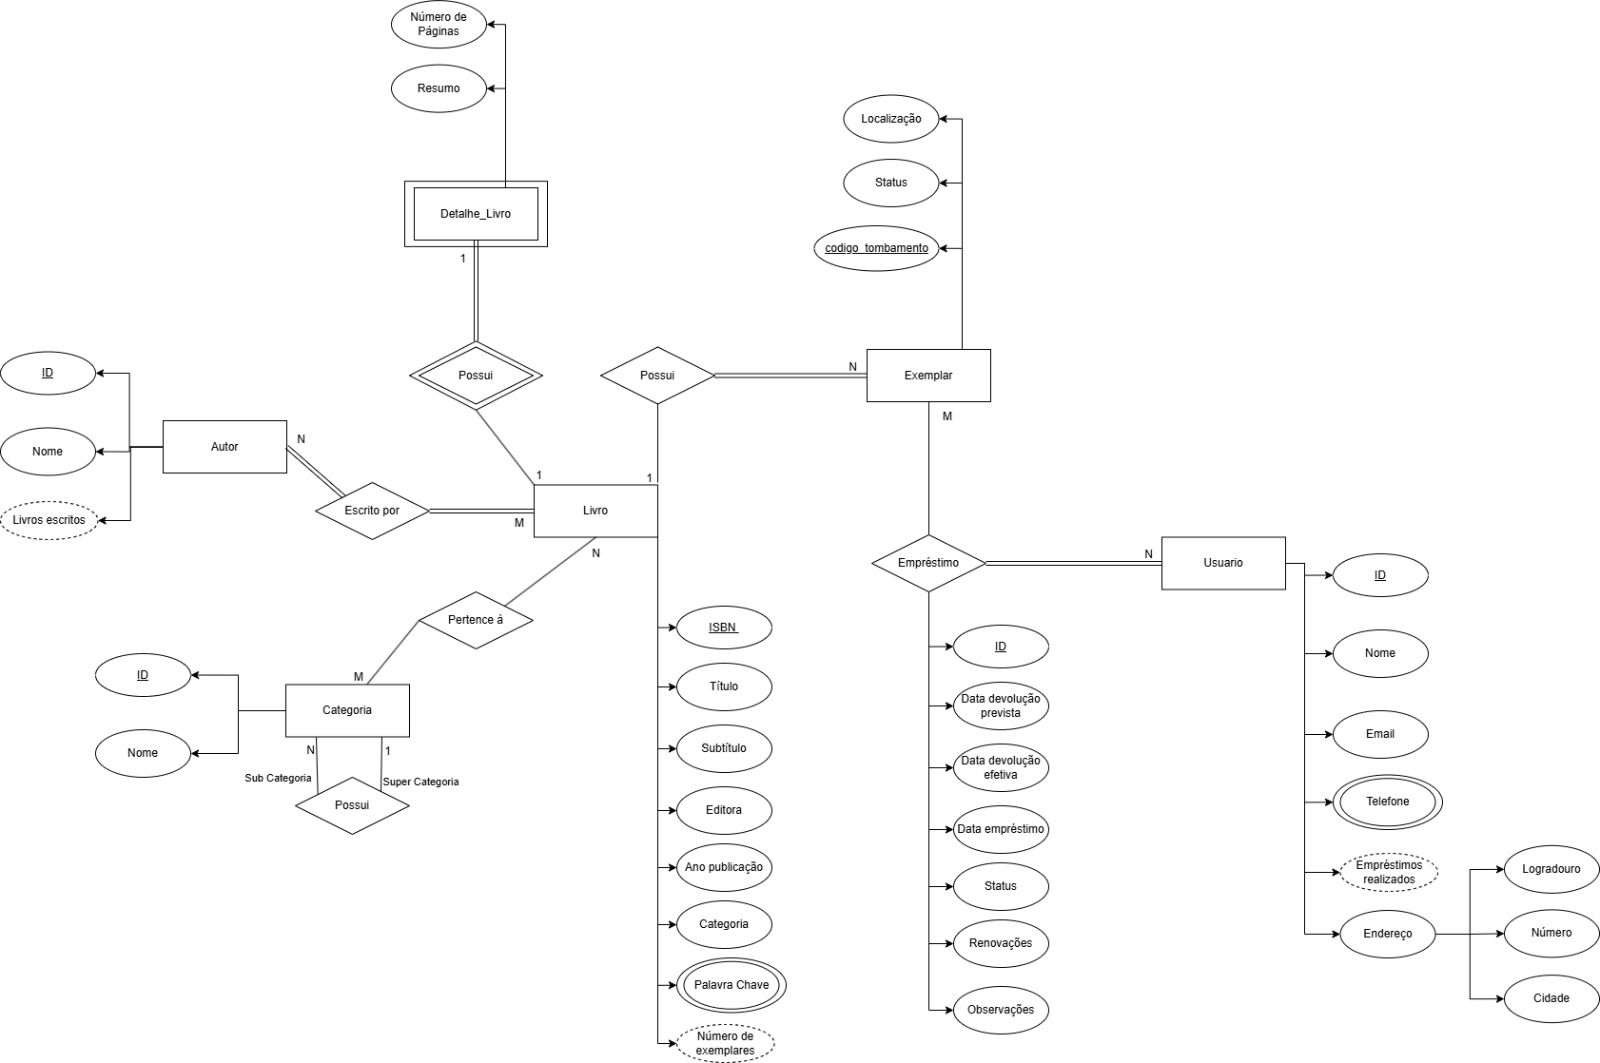
\includegraphics[width=0.95\textwidth]{ModeloConceitual.png}
    \caption{Diagrama Entidade-Relacionamento do Sistema de Biblioteca Universitária}
    \label{fig:diagrama-er}
\end{figure}

%----------------------------------------------------------------------------------------
% RELATIONAL SCHEMA
%----------------------------------------------------------------------------------------
\section{Esquema Relacional}

\subsection{Processo de Mapeamento}

O esquema relacional foi derivado a partir do modelo ER, aplicando um conjunto sistemático de regras de transformação:

\begin{conceptbox}[Estratégias de Mapeamento]
\begin{enumerate}
    \item \textbf{Mapeamento de Entidades Regulares:} Cada entidade se torna uma tabela com seus atributos, onde o identificador se torna a chave primária.
    
    \item \textbf{Mapeamento de Entidades Fracas:} Transformadas em tabelas cujas chaves primárias incorporam a chave primária da entidade forte relacionada.
    
    \item \textbf{Mapeamento de Relacionamentos 1:1:} Implementados através de chaves estrangeiras, geralmente na relação correspondente à entidade com participação total.
    
    \item \textbf{Mapeamento de Relacionamentos 1:N:} Implementados através de chaves estrangeiras na tabela correspondente ao lado "muitos" do relacionamento.
    
    \item \textbf{Mapeamento de Relacionamentos N:M:} Implementados através de tabelas de junção que contêm as chaves primárias das entidades participantes.
    
    \item \textbf{Mapeamento de Atributos Multivalorados:} Transformados em tabelas separadas com chaves estrangeiras referenciando a entidade principal.
    
    \item \textbf{Mapeamento de Auto-relacionamentos:} Implementados através de chaves estrangeiras que referenciam a própria tabela.
\end{enumerate}
\end{conceptbox}

\subsection{Modelo Relacional}

\begin{figure}[H]
    \centering
    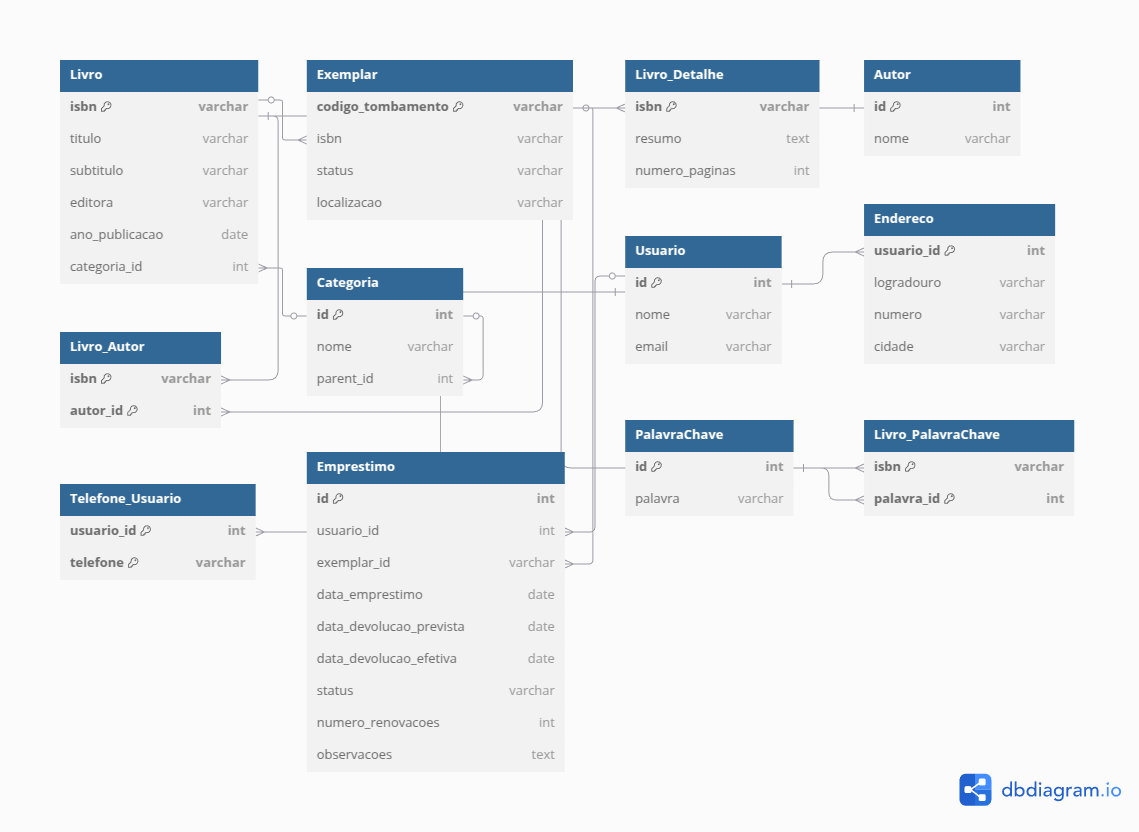
\includegraphics[width=\textwidth]{ModeloRelacional.png}
    \caption{Diagrama do Esquema Relacional do Sistema de Biblioteca}
    \label{fig:modelo-relacional}
\end{figure}

\subsection{Relações Resultantes}

\begin{conceptbox}[Tabelas do Esquema Relacional]
\begin{description}
    \item[Categoria] \hfill \\
    \textbf{(\underline{id}, nome, parent\_id)} \\
    Onde \textit{parent\_id} é uma chave estrangeira que referencia \textit{id} na mesma tabela, implementando o auto-relacionamento hierárquico.
    
    \item[Livro] \hfill \\
    \textbf{(\underline{isbn}, titulo, subtitulo, editora, ano\_publicacao, categoria\_id)} \\
    Onde \textit{categoria\_id} é uma chave estrangeira para a tabela \textbf{Categoria}.
    
    \item[Livro\_Detalhe] \hfill \\
    \textbf{(\underline{isbn}, resumo, numero\_paginas)} \\
    Onde \textit{isbn} é chave primária e estrangeira referenciando a tabela \textbf{Livro}.
    
    \item[Autor] \hfill \\
    \textbf{(\underline{id}, nome)}
    
    \item[Livro\_Autor] \hfill \\
    \textbf{(\underline{isbn, autor\_id})} \\
    Tabela de junção para o relacionamento N:M entre \textbf{Livro} e \textbf{Autor}.
    
    \item[PalavraChave] \hfill \\
    \textbf{(\underline{id}, palavra)}
    
    \item[Livro\_PalavraChave] \hfill \\
    \textbf{(\underline{isbn, palavra\_id})} \\
    Tabela de junção para o relacionamento N:M entre \textbf{Livro} e \textbf{PalavraChave}.
    
    \item[Exemplar] \hfill \\
    \textbf{(\underline{codigo\_tombamento}, isbn, status, localizacao)} \\
    Onde \textit{isbn} é uma chave estrangeira para a tabela \textbf{Livro}.
    
    \item[Usuario] \hfill \\
    \textbf{(\underline{id}, nome, email)}
    
    \item[Endereco] \hfill \\
    \textbf{(\underline{usuario\_id}, logradouro, numero, cidade)} \\
    Onde \textit{usuario\_id} é chave primária e estrangeira referenciando a tabela \textbf{Usuario}.
    
    \item[Telefone\_Usuario] \hfill \\
    \textbf{(\underline{usuario\_id, telefone})} \\
    Onde \textit{usuario\_id} é parte da chave primária e referencia a tabela \textbf{Usuario}.
    
    \item[Emprestimo] \hfill \\
    \textbf{(\underline{id}, usuario\_id, exemplar\_id, data\_emprestimo, data\_devolucao\_prevista,} \\
    \textbf{data\_devolucao\_efetiva, status, numero\_renovacoes, observacoes)} \\
    Onde \textit{usuario\_id} e \textit{exemplar\_id} são chaves estrangeiras para as tabelas \textbf{Usuario} e \textbf{Exemplar}, respectivamente.
\end{description}
\end{conceptbox}

\subsection{Restrições de Integridade}

\begin{conceptbox}[Mecanismos de Integridade]
\begin{itemize}
    \item \textbf{Integridade de Entidade:} Todas as chaves primárias são definidas como NOT NULL, garantindo que cada registro tenha identificação única.
    
    \item \textbf{Integridade Referencial:} Implementada através de FOREIGN KEY constraints entre tabelas relacionadas.
    \begin{itemize}
        \item ON DELETE CASCADE: Aplicado em relações onde a exclusão do registro principal deve propagar para os dependentes (ex: exclusão de usuário propaga para seu endereço).
        \item ON DELETE RESTRICT: Impede a exclusão de registros que possuem dependentes (ex: um livro com exemplares).
    \end{itemize}
    
    \item \textbf{Restrições de Domínio:} Garantem que os dados inseridos nas colunas obedeçam a certos critérios:
    \begin{itemize}
        \item CHECK constraints para validar valores permitidos (ex: status de exemplar)
        \item UNIQUE constraints para campos com unicidade obrigatória (ex: email de usuário)
        \item DEFAULT values para campos com valores padrão (ex: data de empréstimo)
    \end{itemize}
\end{itemize}
\end{conceptbox}

%----------------------------------------------------------------------------------------
% OPERATIONS AND QUERIES
%----------------------------------------------------------------------------------------
\section{Operações e Consultas}

O esquema relacional suporta diversas operações e consultas essenciais para o funcionamento do sistema. A seguir, apresentamos as principais categorias de operações e exemplos das consultas mais relevantes.

\subsection{Gestão do Acervo}

\begin{conceptbox}[Operações de Catalogação]
\begin{enumerate}[label=\textbf{OA\arabic*.}]
    \item \textbf{Cadastro Hierárquico de Categorias}
    \begin{itemize}
        \item Registro de categorias principais (sem parent\_id)
        \item Criação de subcategorias (com referência à categoria pai)
        \item Consulta de árvore de categorias (recursivamente)
    \end{itemize}

    \item \textbf{Registro Completo de Livros}
    \begin{itemize}
        \item Inserção de informações bibliográficas básicas
        \item Cadastro de detalhes complementares
        \item Associação com autores existentes
        \item Indexação por palavras-chave
    \end{itemize}

    \item \textbf{Gestão de Exemplares}
    \begin{itemize}
        \item Registro de novas cópias físicas
        \item Atualização de status e localização
        \item Verificação de disponibilidade
    \end{itemize}
\end{enumerate}
\end{conceptbox}

\begin{conceptbox}[Consultas do Acervo]
\begin{enumerate}[label=\textbf{CA\arabic*.}]
    \item \textbf{Busca Multidimensional de Livros}
    \begin{itemize}
        \item Por categoria (incluindo subcategorias)
        \item Por autor (nome completo ou parcial)
        \item Por palavras-chave
        \item Por disponibilidade de exemplares
    \end{itemize}

    \item \textbf{Relatórios de Composição do Acervo}
    \begin{itemize}
        \item Distribuição de livros por categoria
        \item Quantidade de exemplares por título
        \item Estado de conservação do acervo
    \end{itemize}
\end{enumerate}
\end{conceptbox}

\subsection{Gestão de Usuários}

\begin{conceptbox}[Operações de Usuários]
\begin{enumerate}[label=\textbf{OU\arabic*.}]
    \item \textbf{Gerenciamento de Cadastros}
    \begin{itemize}
        \item Inserção de novos usuários com validação de email
        \item Registro de endereço completo
        \item Cadastro de múltiplos telefones
        \item Atualização de informações pessoais
    \end{itemize}

    \item \textbf{Consultas de Usuários}
    \begin{itemize}
        \item Busca por dados de identificação (ID, nome, email)
        \item Recuperação de informações completas (inclui endereço e telefones)
        \item Verificação de histórico e situação atual
    \end{itemize}
\end{enumerate}
\end{conceptbox}

\subsection{Gestão de Empréstimos}

\begin{conceptbox}[Operações de Circulação]
\begin{enumerate}[label=\textbf{OC\arabic*.}]
    \item \textbf{Controle de Empréstimos}
    \begin{itemize}
        \item Registro de novas operações com validação de regras
        \item Verificação de empréstimos ativos por usuário
        \item Identificação de situação (regular ou atrasado)
    \end{itemize}

    \item \textbf{Gestão de Devoluções}
    \begin{itemize}
        \item Registro da data efetiva de retorno
        \item Atualização de status do empréstimo e exemplar
        \item Cálculo automático de atraso
    \end{itemize}

    \item \textbf{Renovações}
    \begin{itemize}
        \item Extensão do prazo de devolução
        \item Incremento do contador de renovações
        \item Verificação de limites e restrições
    \end{itemize}
\end{enumerate}
\end{conceptbox}

\subsection{Relatórios e Análises}

\begin{conceptbox}[Consultas Analíticas]
\begin{enumerate}[label=\textbf{RA\arabic*.}]
    \item \textbf{Indicadores de Utilização}
    \begin{itemize}
        \item Ranking de livros mais emprestados
        \item Distribuição de empréstimos por categoria
        \item Análise temporal de circulação
    \end{itemize}

    \item \textbf{Monitoramento de Atrasos}
    \begin{itemize}
        \item Identificação de empréstimos com devolução em atraso
        \item Ranking de usuários por frequência de atrasos
        \item Tempo médio de atraso por categoria de usuário
    \end{itemize}

    \item \textbf{Eficiência do Acervo}
    \begin{itemize}
        \item Taxa de circulação por categoria
        \item Relação entre quantidade de exemplares e empréstimos
        \item Análise de autores e temas mais populares
    \end{itemize}
\end{enumerate}
\end{conceptbox}

%----------------------------------------------------------------------------------------
% CONCLUSION
%----------------------------------------------------------------------------------------
\section{Conclusão}

O Sistema de Gerenciamento de Biblioteca Universitária aqui documentado representa uma solução robusta para as necessidades de controle e operação de bibliotecas acadêmicas. Através de um modelo de dados bem estruturado, o sistema permite:

\begin{infobox}
\begin{itemize}
    \item \textbf{Catalogação Eficiente:} Organização hierárquica do acervo com categorização flexível e indexação por múltiplos critérios.
    
    \item \textbf{Circulação Controlada:} Gestão completa do ciclo de empréstimos, com monitoramento de prazos e controle de disponibilidade.
    
    \item \textbf{Gestão de Usuários:} Cadastro completo com informações pessoais e histórico de utilização dos serviços.
    
    \item \textbf{Inteligência Analítica:} Relatórios e consultas que auxiliam na tomada de decisão e otimização do acervo.
\end{itemize}
\end{infobox}

A abordagem adotada seguiu as melhores práticas de modelagem de dados, iniciando com a análise do minimundo, passando pelo desenvolvimento do modelo conceitual (ER) e culminando no esquema relacional normalizado. O resultado é um banco de dados que equilibra eficiência operacional, integridade de dados e flexibilidade para expansões futuras.

A implementação deste sistema proporcionará significativa melhoria na gestão bibliotecária, beneficiando tanto os profissionais responsáveis pela administração quanto a comunidade acadêmica que utiliza estes recursos.

\end{document}